\documentclass[12pt]{article}
\usepackage[T1]{fontenc}
\usepackage[utf8]{inputenc}
\usepackage{polski}
\usepackage{minted}
\usepackage{geometry}
\usepackage{natbib}
\usepackage{enumitem}
\usepackage{graphicx}
\usepackage{bold-extra}
\usepackage[font=small,labelfont=bf]{caption}
\usepackage{hyperref}
\usepackage{titlesec}
\usepackage{indentfirst}
\hyphenpenalty=10000
\tolerance=1000 \emergencystretch=2em
\titlelabel{\thetitle.\quad}

 \geometry{
     left=23mm,
     top=25mm,
     right=23mm
 }


\def\mydate{\leavevmode\hbox{\twodigits\day.\twodigits\month.\the\year}}
\def\twodigits#1{\ifnum#1<10 0\fi\the#1}

\begin{document}
%titlepage
\thispagestyle{empty}
\begin{center}
\begin{minipage}{0.75\linewidth}
    \centering
    
\includegraphics[width=0.45\linewidth]{agh_logo2.png}
    \par
    \vspace{2cm}
    {\bfseries{\scshape{\Huge  Teoria współbieżności}}}
    \par
    \vspace{1.7cm}
    {\scshape{\Large Laboratorium 10}}
    \par
    \vspace{0.8cm}
    {\scshape{\Large Teoria śladów}}
    \par
    \vspace{3cm}

    {\scshape{\Large Albert Gierlach}}\par
    \vspace{1cm}

    {\Large \mydate}
\end{minipage}
\end{center}
\clearpage



\section{Zadanie 1}
Rozważmy zbiór zmiennych („bazę danych”) {x, y, z} i następujący zbiór akcji („transakcji”) modyfikujących wartości tych zmiennych:
\[ (a)\;x := x + y \]
\[ (b)\;y := y + 2z \]
\[ (c)\;x := 3x + z \]
\[ (d)\;z := y - z \]

Akcje możemy wykonywać współbieżnie z następującym zastrzeżeniem: akcja zmieniająca wartość zmiennej nie może być wykonana współbieżnie z akcją odczytującą lub modyfikującą stan tej samej zmiennej. W języku teorii śladów: dwie akcje są zależne jeśli obie operują na tej samej zmiennej, a przynajmniej jedna z nich modyfikuje wartość tej zmiennej.
 
 
\begin{enumerate}[label=\alph*)]
    \item W alfabecie A = { a, b, c, d} określ relacje zależności i niezależności.
    \item Wyznacz ślad wyznaczony przez słowo w = baadcb względem powyższej relacji niezależności.
    \item Wyznacz postać normalną Foaty śladu [w]
    \item Narysuj graf zależności Diekerta (w postaci zminimalizowanej - bez krawędzi "przechodnich") dla słowa w.
\end{enumerate} 

\section{Rozwiązanie}
\noindent
a) Relacja zależności:
\[ D = \{(a, a),(a, b),(a, c),(b, a),(b, b),(b, d),(c, a),(c, c),(c, d),(d, b),(d, c),(d, d)\}  \]

Relacja niezależności:
\[ I = \{(a, d),(d, a),(b, c),(c, b)\}  \]

\vspace{0.4cm}
\noindent
b) Śladem słowa baadcb względem relacji niezależności jest:
\[ [baadcb]_I = \{ baadcb, badacb, baadbc, badabc, bdaabc, bdaacb \} \]
\noindent
wynika to z faktu, iż możemy zamienić kolejność sąsiednich operacji, jeżeli są one niezależne od siebie, dzięki temu otrzymujemy sześć możliwych permutacji rozważanego słowa.

\newpage
\noindent
c) Korzystając z podanego algorytmu wyznaczyłem postać normalną Foaty dla śladu [w], która wygląda następująco:
\[  [w] = (b)(ad)(a)(bc)  \]

\vspace{0.4cm}
\noindent
d) graf Diekerta dla słowa "baadcb":
\begin{center}
\centering
    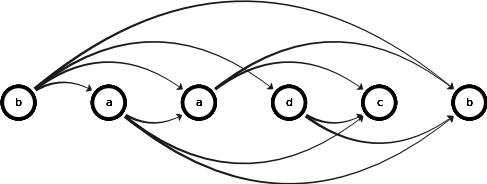
\includegraphics{graph1.png}
    \captionof{figure}{Graf Diekierta}
\end{center}

\noindent
Krawędzie przechodnie w tym grafie to: (b, b), (b, a), (a, c), (a, b)

\begin{center}
\centering
    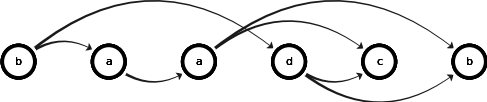
\includegraphics{graph1_reduced.png}
    \captionof{figure}{Graf Diekierta bez krawędzi przechodnich}
\end{center}

\newpage
\noindent
Graf w bardziej czytelnej postaci:
\begin{center}
\centering
    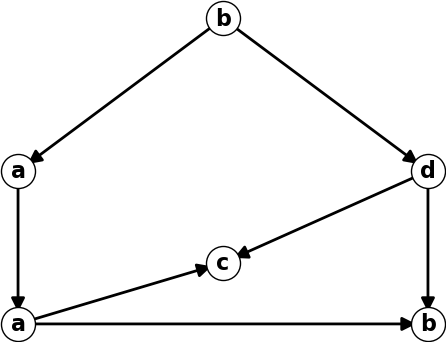
\includegraphics[scale=0.6]{graph1_reduced_pretty.png}
    \captionof{figure}{Graf Diekierta dla słowa baadcb}
\end{center}

\section{Zadanie 2}
Dany jest zbiór akcji:

\[ (a)\;x := y + z \]
\[ (b)\;y := x + w + y \]
\[ (c)\;x := x + y + v \]
\[ (d)\;w := v + z \]
\[ (e)\;v := x + v + w \]
\[ (f)\;z := y + z + v \]

\begin{enumerate}[label=\alph*)]
    \item W alfabecie A = { a, b, c, d, e, f} określ relacje zależności i niezależności.
    \item Wyznacz postać normalną Foaty śladu [u], u = acdcfbbe
    \item Narysuj graf zależności Diekerta (w postaci zminimalizowanej - bez krawędzi "przechodnich") dla słowa u.
\end{enumerate} 

\newpage
\section{Rozwiązanie}
\noindent
a) Relacja zależności:
\[
\begin{array}{c}
D = sym\{ 
(a, a), (a, b), (a, c), (a, e), (a, f), (b, b), (b, c), (b, d), (b, f), \\
(c, c), (c, e), (d, d), (d, e), (d, f), (e, e), (e, f) (f, f)
\}
\end{array}
\]

Relacja niezależności:
\[ I = sym\{(a, d), (b, e), (c, d), (c, f)\}  \]

\noindent
b) Korzystając z podanego algorytmu wyznaczyłem postać normalną Foaty dla śladu [u], która wygląda następująco:
\[  [u] = (ad)(cf)(c)(be)(b)  \]

\noindent
c) graf Diekerta (po usunięciu krawędzi przechodnich) dla słowa "acdcfbbe":

\begin{center}
\centering
    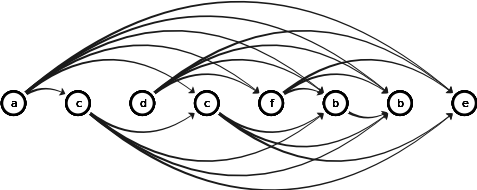
\includegraphics{graph2.png}
    \captionof{figure}{Graf Diekierta}
\end{center}

\noindent
Krawędzie przechodnie w tym grafie to: (a, e), (d, e), (c, b), (a, c), (f, b), (a, b), (c, e), (d, b), (a, b), (c, b), (c, b), (d, b)

\begin{center}
\centering
    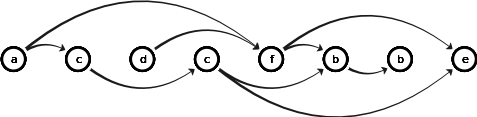
\includegraphics{graph2_reduced.png}
    \captionof{figure}{Graf Diekierta bez krawędzi przechodnich}
\end{center}

\noindent
Graf w bardziej czytelnej postaci:
\begin{center}
\centering
    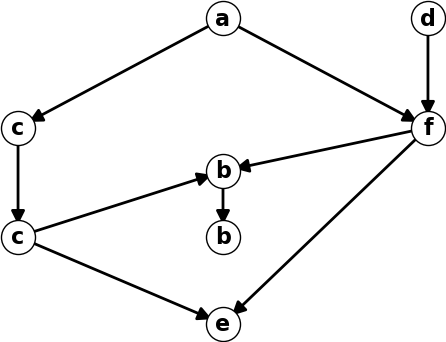
\includegraphics[scale=0.6]{graph2_reduced_pretty.png}
    \captionof{figure}{Graf Diekierta dla słowa acdcfbbe}
\end{center}


\section{Bibliografia}
\begin{itemize}
    \item \url{http://citeseerx.ist.psu.edu/viewdoc/download?doi=10.1.1.38.4401&rep=rep1&type=pdf}
    \item \url{https://en.wikipedia.org/wiki/Trace_theory}

\end{itemize}

\end{document}
